\chapter{Model}
\label{Model}

A model has been made with two goal of answering two questions:
\begin{itemize}[itemsep=-1ex,topsep=0pt]
	\item How strong are the reflections of flashes in a realistic environment?
	\item How and how much, will these reflections change if an object enters the illuminated area
\end{itemize}
This section uses the model explained in section \ref{Model_explained}. It starts with what changes where made in the presented model, in comparison to the original \cite{Advances_In_Optical_Communication} and shows that the model gives a reasonable estimation of reality. It then describes two modelled scenarios and presents the results. The chapter ends with answering the posed questions.

\section{Model description}
The model made is an interpretation of the Phong reflection model (see section \ref{Model_explained}). It calculates how much of the light leaving a luminaire, bounces back via the environment to a photo diode placed next to the light source. This section will first discuss the adjustments made to the Phong model, followed by an explanation of the simulation process.

\subsection{Model Adjustments}
The model presented in section \ref{Model_explained} is not the complete Phong model. Several parts where simplified or removed as they should barely influence the results of the simulation.

The first adjustment is the removal of "time". The methods in the literature took the travelling time of light into account in order to calculate the possible inter-symbol interference. This is not required for this simulation as we are only interested in the steady state situation when the light is fully turned on and the light received by the photo diode is maximized for the current situation.

The second adjustment is the removal of "colour". The original method differentiated between different wavelengths of visible light, while producing, reflecting and receiving light. It was therefore maintaining colour information. This is however not necessary for this model, as we do not care about the colour of the reflecting objects, but only about the total amount of energy reflected by the object. For this reason, the surface reflection coefficient ($p(\lambda)$) was replaced with the albedo of the object instead ($A$).
\begin{equation}
\label{Model_simp_2}
\Gamma = \int_{380nm}^{780nm} \Phi_e p(\lambda) d\lambda \to \Gamma = \Phi_{lum} A
\end{equation}

Albedo is a property of an object representing the ratio of energy which is reflected when sun is shining on it. Even though albedo is based on the full spectrum of sunlight instead of only the wavelengths of visible light, it gives a reasonable approximation of the reflection coefficient in this scenario. This is shown in section \ref{sec:verification}.

The final adjustment is the amount of reflections we calculate. In reality a light ray can be reflected an infinite amount of times of off several different surfaces before returning back to the sensor. In the model however we only calculated one bounce (from the light to an object and back). The reason for this is that the first reflection provides approximately 80\% of the signal where all other reflections only make up 20\% of the total power\cite{indoor_VLC_no_LOS}. If we where to add multiple bounces, the accuracy of the model would only increase by a maximum 20\%. Adding the extra bounces makes the model many more times complicated, depended on the environment we are simulating. A simple hallway model would be 8 times as complex to model and require at least 4 times as much computation power, while only providing "only" 16\% more accuracy.

\subsection{Calculation process}
Calculating the amount of light reflecting back to the object is a three step process. The first step is to calculate the shadow casted by the object on the floor and walls. This is required as the surface where the shadow is casted can't reflect light back directly to the photo diode. It's important to note that the light casting the shadow is reflected of the object instead and with that, changes the reflection pattern of the room.

The second step is to calculate how much light reflected from all floors and walls (where no shadow is casted) is received by the photo diode. The final step is to calculate how much light is reflected from each side of the object. \ref{fig:raytracing} shows an overview of an environment with rays leaving the light, casting shadow and the resulting reflections.

\begin{figure}
	\centering     %%% not \center
	\subfigure[Sideview]{\label{fig:Calculation_frontview}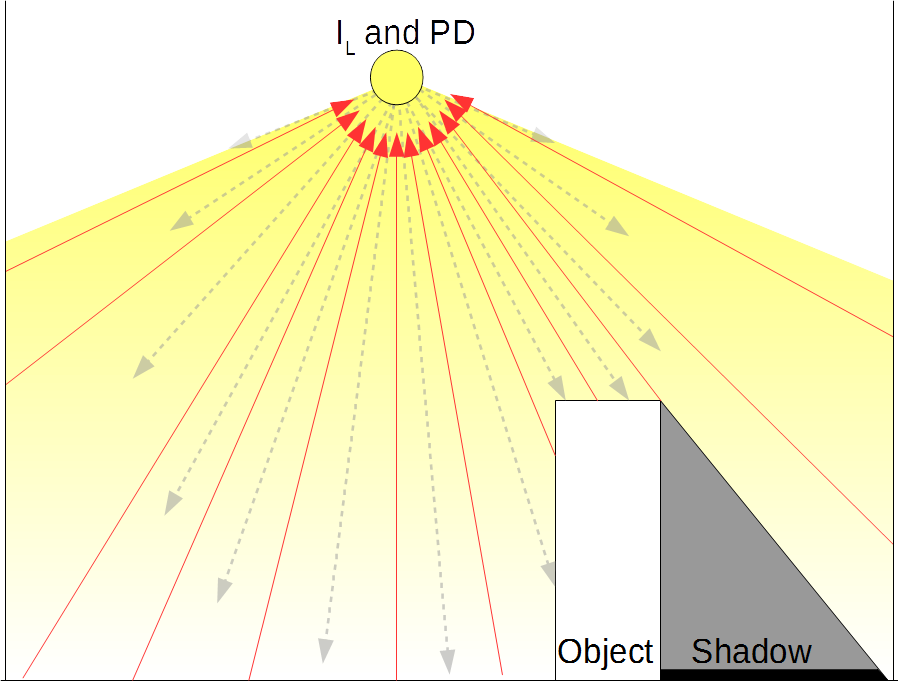
\includegraphics[width=68mm]{pics/Calculation_frontview.png}}
	\subfigure[Topview]{\label{fig:Calulation_topview}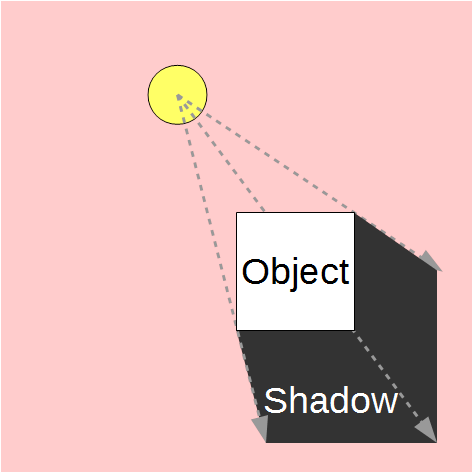
\includegraphics[width=52mm]{pics/Calulation_topview.png}}
	\caption{Overview of the calculation process. Grey lines represent light rays casted by the light. Black represents the shadow casted by the object on the floor or walls. Red lines or areas show reflections bouncing from the ground, walls or object back to the photo diode.\label{fig:raytracing}}
\end{figure}

\section{Verification}
\label{sec:verification}
The calculation method and changes in the model where verified using a scale model featuring a LED\cite{lamptest}, a paper box and a light meter\cite{LuxMeter}. The first step of verifying the model is to check if the LED is modelled properly by equation \ref{eq:I(phi)}. This was done by hanging the LED at 100cm above the floor and measuring the horizontal illuminance ($E_{hor}$) at the floor to see if the measured irradiation pattern of the LED matches the theoretical pattern produced by equation \ref{eq:E_hor}. Measurements and simulations in Appendix \ref{app_repository} show that the LED in the test set-up was producing more light than in the specification. These numbers where therefore adjusted for the next step of verification.

The second step is the verification of the interpretation of the Phong model. This was done with the test set-up shown in Figure \ref{fig:VerificationSetup}. By moving a paper box across a paper covered floor in steps of 5cm and measuring the reflections in each step, we obtain the red line in figure \ref{fig:verf_paper}. When we compare this line with the blue line generated by the model using $A = 0.75$ (albedo of paper according to \cite{Albedo}), then the lines closely match.

The test was repeated while the using the original floor of the room. The albedo of the floor was calculated to be 0.37, based on a measurement of the floor without the paper box. The result of the second test can be seen in Figure \ref{fig:verf_floor}. The resulting curves also seem similar. As the model has shown to be reflect reality quite closely, it seems fine to assume that the model works and can be trusted some extend. It won't give exact results, but it will al least provide a proper approximation of the perceived light.

\begin{figure}[]
	\centering
	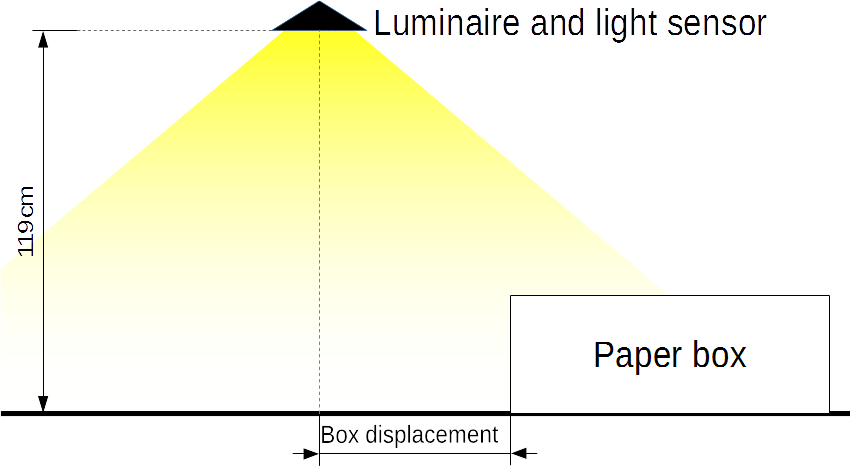
\includegraphics[width=\textwidth]{pics/Verification_Situation.png}
	\caption{Visualisation of the model verification set-up.\label{fig:VerificationSetup}}
\end{figure}

\begin{figure}
	\centering     %%% not \center
	\subfigure[]{\label{fig:verf_paper}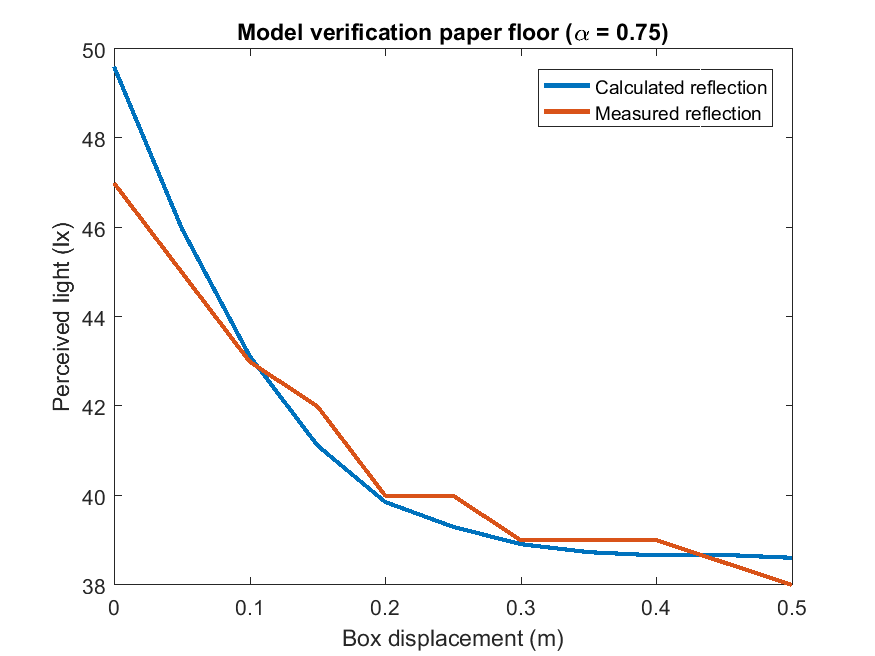
\includegraphics[width=60mm]{pics/ModelVerificationResults_paper.png}}
	\subfigure[]{\label{fig:verf_floor}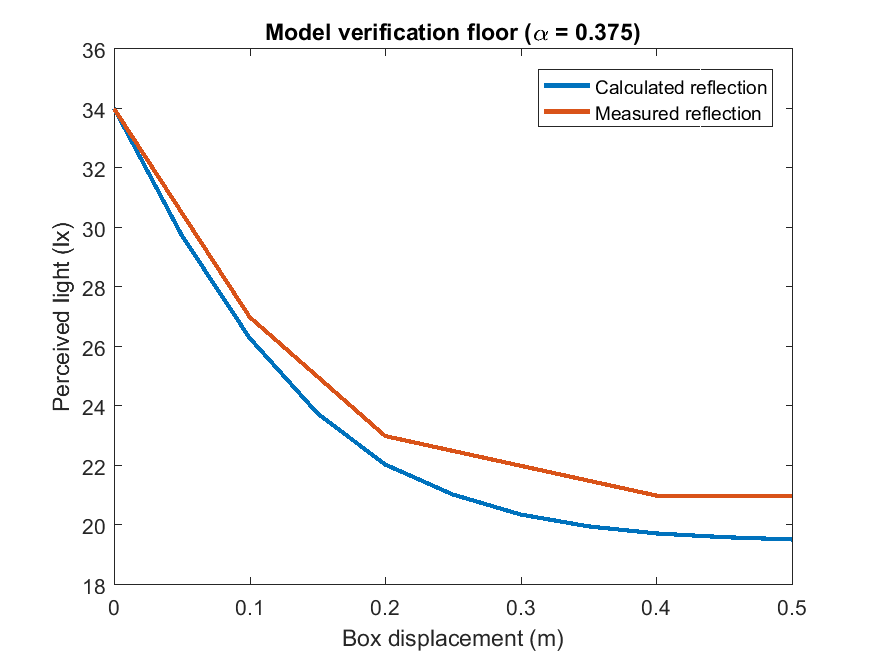
\includegraphics[width=60mm]{pics/ModelVerificationResults_floor.png}}
	\caption{Both figures show that the model provides a reasonable approximation of the reality. Note that the albedo of paper was taken from \cite{Albedo} and the albedo of the floor was estimated with measurements.\label{fig:VerificationResults}}
\end{figure}

\section{Modelling of the hallway}
\label{sec:moddelingofthehallway}
The hallway modelled is based on a real hallway located at the TU Delft. The hallway is 2.2m wide and 2.8m high. The floors albedo is set at 0.37, as this was calculated during the verification of the model. The albedo of the walls was set to 0.95 which represents the albedo of white plaster\cite{Albedo}. The reflection of these surfaces is assumed to be fully diffuse ($r_d = 1$).

Industry standards state that corridors in education buildings should be illuminated with at least $E_{mean} > 100lx$ and a light uniformity of $U_o > 0.4$\cite{lichthandbuch}. $E_{mean}$ represents the mean illumination level of the floor and $U_o$ the proportional difference between $E_{mean}$ and $E_{minimum}$. These lighting requirements can be achieved using the same luminaire used during the verification process if hung in the staggered formation shown in figure \ref{fig:pattern_hallway}. Calculations showing that the industry standards are met can be found in Appendix \ref{app_repository}.

\begin{equation}
\label{Emean_and_Uo}
	E_{mean} = \frac{1}{y \cdot x}\int_y \int_x E_{hor}(x,y) dy dx
\qquad
	U_o = \frac{E_{mean}}{E_{minimum}}
\end{equation}

The object passing by the light (representing a human) will be modelled as a cuboid 0.2m wide and 0.5m long with varying heights. Several albedos have been assigned to the cuboid to represent the different kind of clothing humans wear. The object will be moved in a straight line trough the hallway with the light at a set vertical distance $y$. Some example paths can be seen in Figure \ref{fig:traveling_path}.

\begin{figure}
	\centering     %%% not \center
	\subfigure[Staggerd hallway LED pattern ]{\label{fig:pattern_hallway}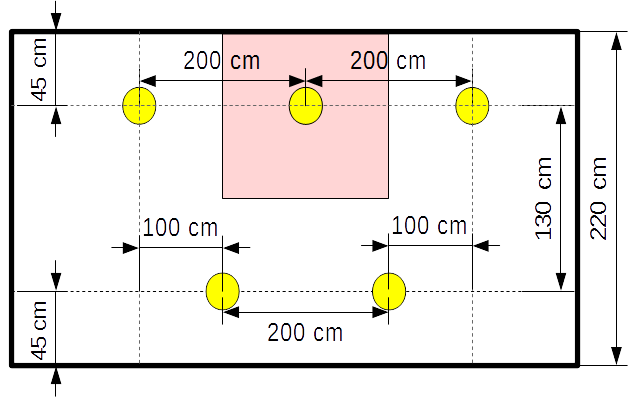
\includegraphics[width=60mm]{pics/LightsOverview.png}}
	\subfigure[Traveling path of the object ]{\label{fig:traveling_path}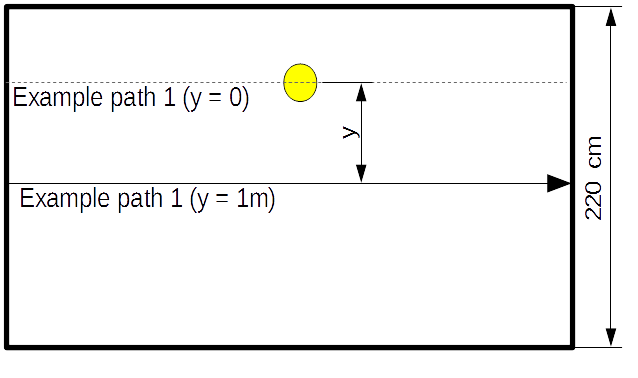
\includegraphics[width=60mm]{pics/TravelingPath.png}}
	\caption{Figure (a) shows the position of the luminaires to obtain a realistic illumination pattern. The red square represents the area one light/photo diode pair should cover. Figure (b) shows an example travelling path of an object.}
\end{figure}

\section{Modelling of the street}
The street model is based on a real street near the TU delft. It has two lanes for cars (each 3m wide) and sidewalk (2m wide). The albedo of the street will be modeled with $A = 0.11$ which represents old asphalt\cite{Albedo}. The reflections of the street are assumed to be fully diffuse ($r_d = 1$).

Industry standards state that a street with side walk should be illuminated with at least $E_{mean} > 3lx$ and a light uniformity of $U_o > 0.2$ \cite{HandboekBestaandeBouw}.These lighting requirements can be achieved using 700lx luminaires with a half power angle of $60^{\circ}$ ($\alpha = 1$) placed every 15 meter in between the road and side walk. This set-up is visualized in figure \ref{fig:pattern_street}. Calculations showing that the industry standards are met can be found in Appendix \ref{app_repository}.

In this model two different objects will be modelled representing humans (walking on the side walk) and cars (driving in the two driving lanes). The humans will be modelled in the same way as in the hallway scenario. The car will be modelled as a cuboid with the dimensions of an Opel Corsa (4m x 1,7m x 1,5m), a commonly seen small car. The objects where modelled with diffuse reflection, because no reliable sources describing the reflection parameters ($r_d$ and $\alpha$) of cars could be found.

Lacking the specular and spread reflections for this specific model should not influence the results significantly, as no part of the car will be moved directly underneath the light and therefore no significant amount of light of the spread reflection should ever reach the light sensor. This is visualized in figure \ref{fig:streetnospecular}.

\begin{figure}
	\centering     %%% not \center
	\subfigure[Topview of the street model ]{\label{fig:pattern_street}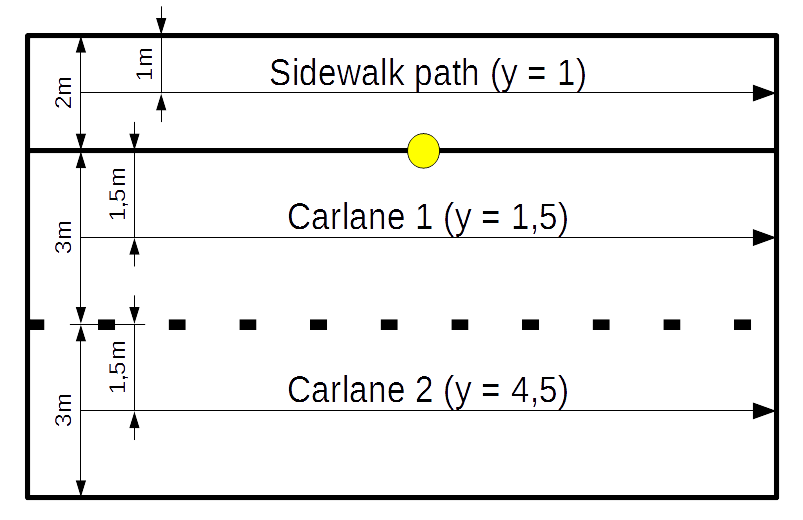
\includegraphics[width=70mm]{pics/TravelingPath_street.png}}
	\subfigure[Spread reflection on cars ]{\label{fig:streetnospecular}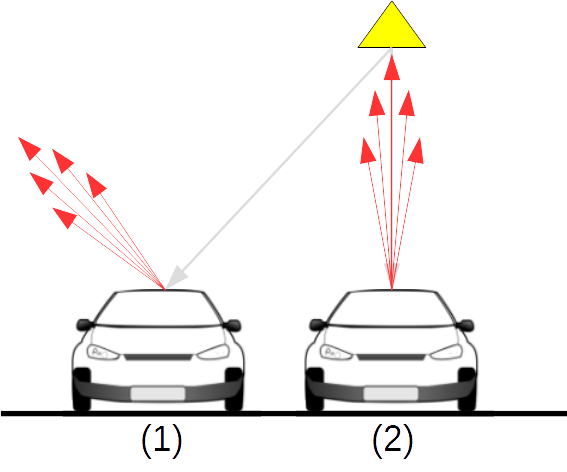
\includegraphics[width=50mm]{pics/StreetNoSpecular.png}}
	\caption{Figure (a) shows an overview of the model. Figure (b) shows that a spread (or specular) reflection will only reach the light in situation (2). This situation does not occur in the modelled scenario.}
\end{figure}

\section{Results}
Several simulated measurements have been graphed in Figure \ref{modelplots}.  All plots can be observed with the tools stored in appendix \ref{app_repository}. The plots on the left side of Figure \ref{modelplots} show the best (most deviation from steady state) and worst case (least deviation from steady state) scenarios for the simulated situations. 

In general we can state that the extremer the albedo, the better the bypassing object can be observed. A high albedo leads to a huge peak in the signal. A low albedo leads to a huge drop in signal as most of the light otherwise bouncing back to the source, is now absorbed by the object itself. Another thing which can be observed is that the smaller the $y$ distance, the more better the signal can be observed.

Figures \ref{fig:humanhallway1FFT}, \ref{fig:humanhallway2FFT}, \ref{fig:humanstreetFFT} and \ref{fig:carstreetFFT}, show the frequency spectrum of the received signals. They where obtained by calculating a Fast Fourier Transfrom (FFT) over the signal with an $F_s$ (sample rate) by assuming a constant movement speed, $5km/h$ for humans and $30km/h$ for cars, over the observed area. These plots show that the frequencies, carrying the signals, lie between 0 and 2Hz for all simulated cases.

\begin{figure}
	\centering     %%% not \center
	\subfigure[]{\label{fig:humanhallway1RSS}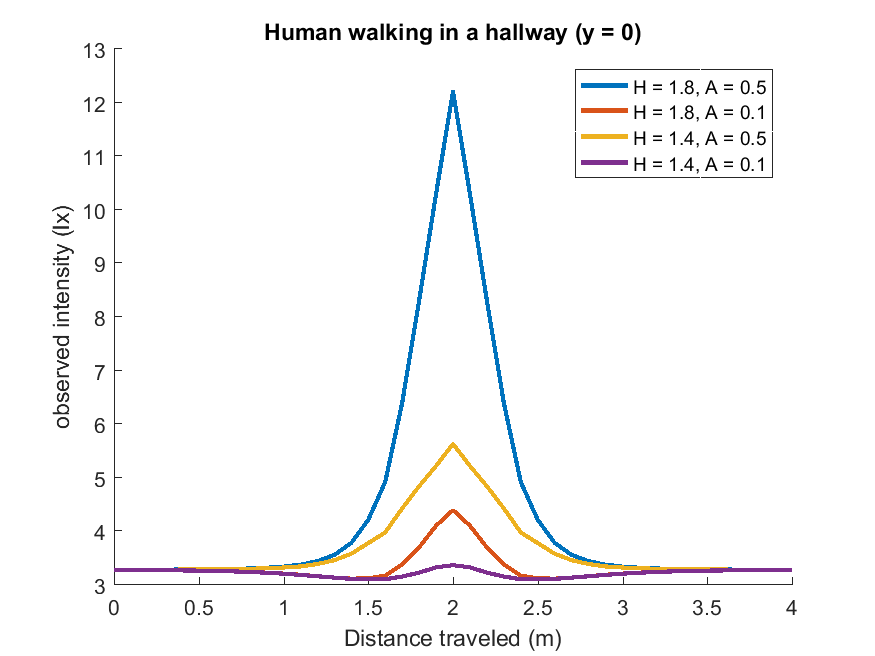
\includegraphics[width=60mm]{pics/Human_hallway1_RSS.png}}
	\subfigure[]{\label{fig:humanhallway1FFT}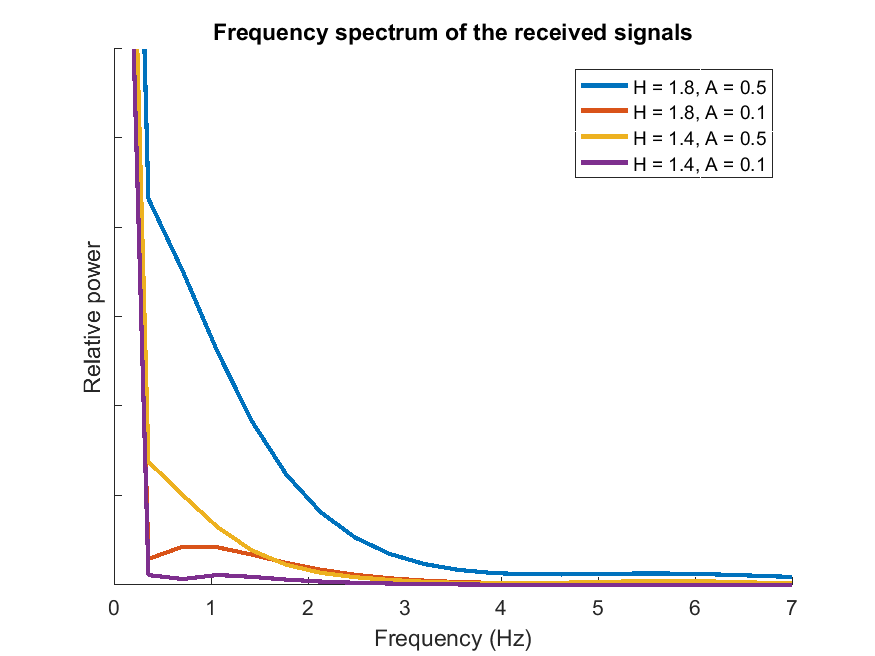
\includegraphics[width=60mm]{pics/Human_hallway1_FFT.png}}	
	\\		\subfigure[]{\label{fig:humanhallway2RSS}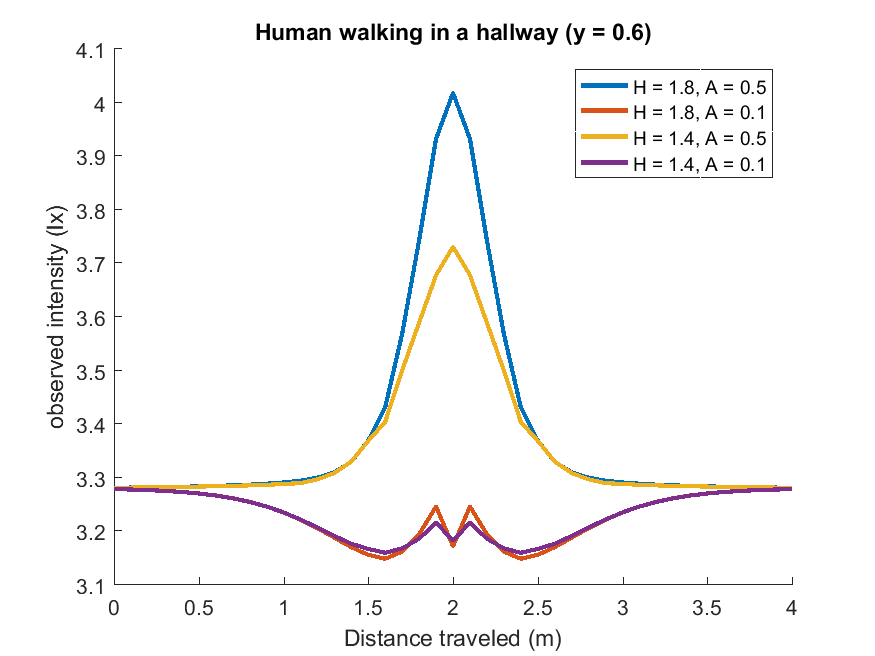
\includegraphics[width=60mm]{pics/Human_hallway2_RSS.png}}
	\subfigure[]{\label{fig:humanhallway2FFT}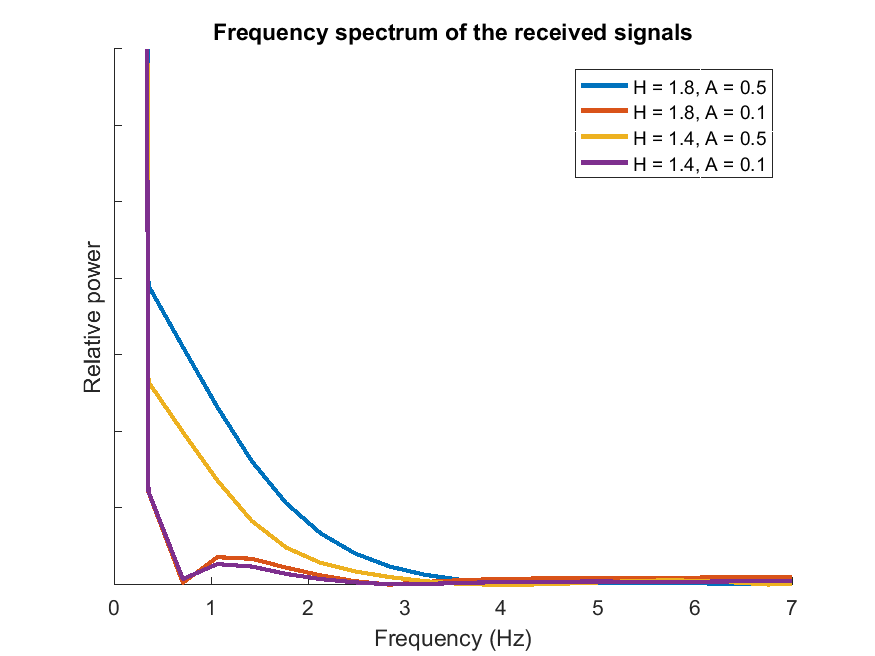
\includegraphics[width=60mm]{pics/Human_hallway2_FFT.png}}	
	\\
	\subfigure[]{\label{fig:humanstreetRSS}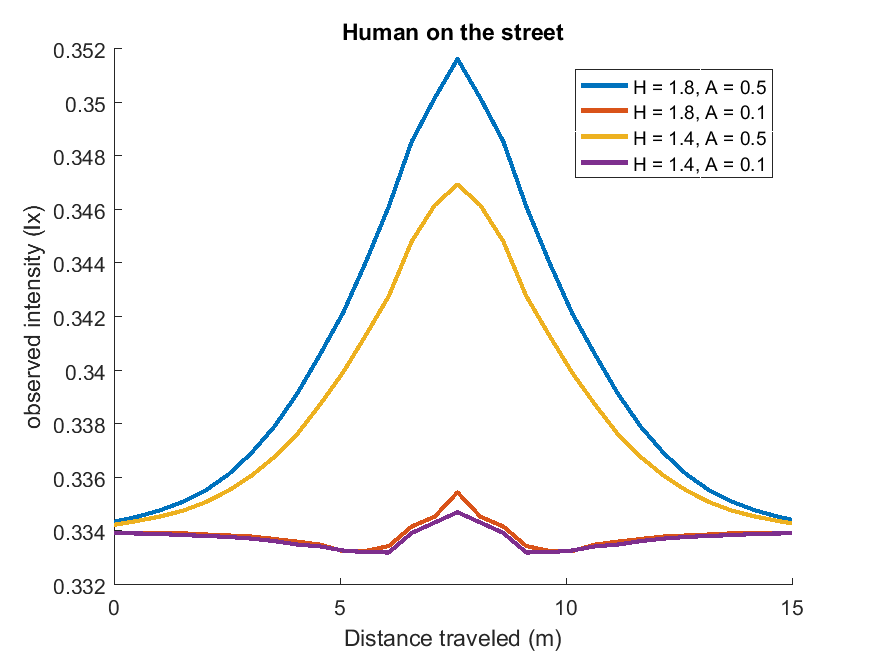
\includegraphics[width=60mm]{pics/Human_street_RSS.png}}
	\subfigure[]{\label{fig:humanstreetFFT}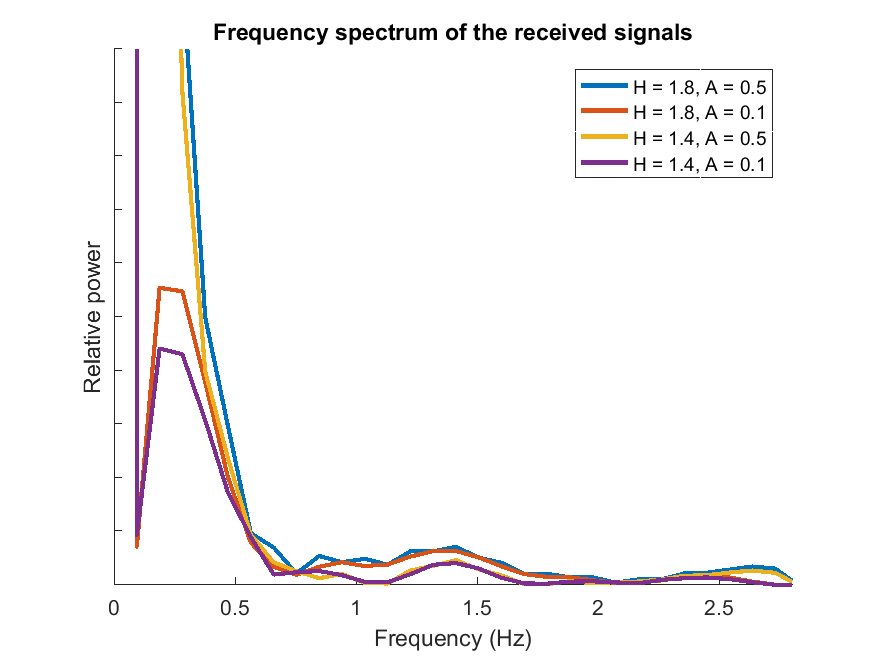
\includegraphics[width=60mm]{pics/Human_street_FFT.png}}
	\\
	\subfigure[]{\label{fig:carstreetRSS}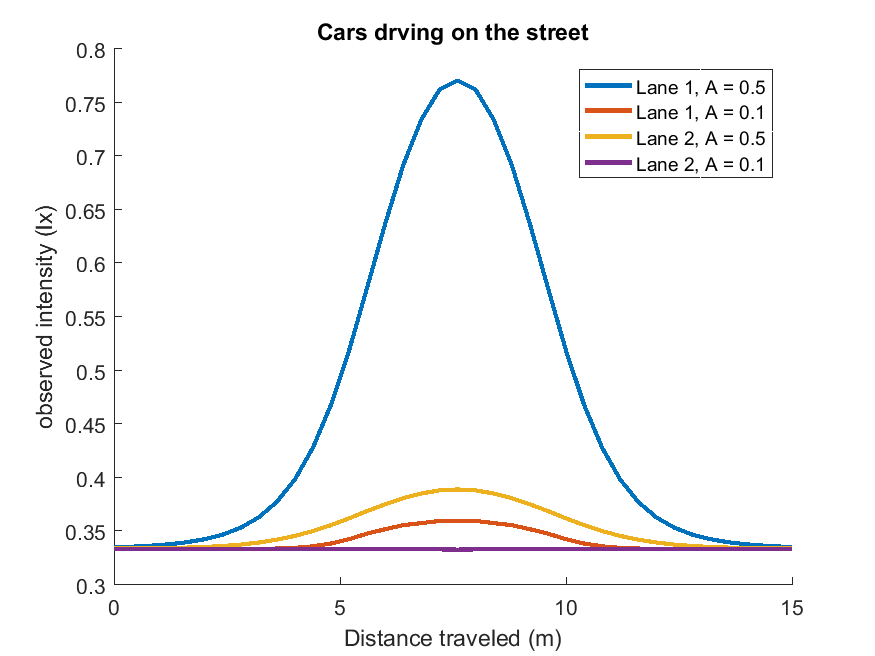
\includegraphics[width=60mm]{pics/Car_street_RSS.png}}
	\subfigure[]{\label{fig:carstreetFFT}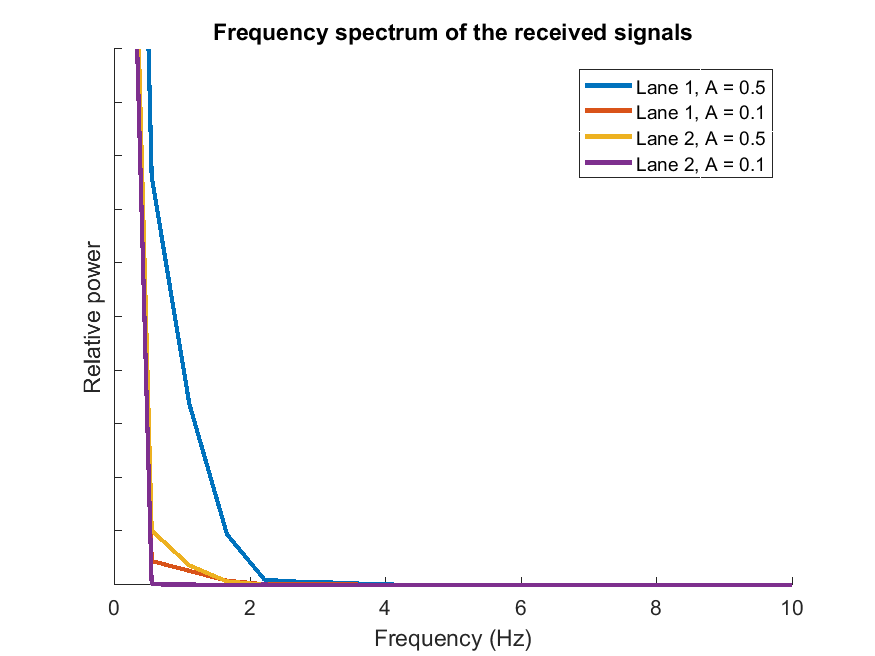
\includegraphics[width=60mm]{pics/Car_street_FFT.png}}
	\caption{Several selected simulated responses. The left figures show the biggest and smallest responses. The right figures show the frequency spectrum of those signals.\label{modelplots}}
\end{figure}

\section{Conclusions}
% An interpertation of the phong model has been made and showed that this works
In this chapter, a version of the Phong model was implemented, verified and used to estimate the light response if a person or car would move past a light/photo diode pair. These responses gave several insights:
\begin{itemize}[itemsep=-1ex,topsep=0pt]
	\item The extremer the albedo, the better an event can be observed.
	\item The bigger the object, the better it can be observed.
	\item The smaller the distance to the light, the better the bypassing object can be observed.
	\item The expected frequency of the signal lies between 0 and 2Hz for both the street and the hallway scenario, no matter what properties the object has.
	\item Building one device which works in both scenarios will be hard, as the expected reflection strengths lie far apart.

\end{itemize}
The insights obtained with this model will be used in several places later on in the thesis.